% !Mode:: "TeX:UTF-8"
\chapter{luaVM}

\section{lua简介}

Lua是一个小巧的脚本语言。由巴西里约热内卢天主教大学
(Pontifical Catholic University of Rio de Janeiro)里的一个研究小组,
由Roberto Ierusalimschy、Waldemar Celes 和 Luiz Henrique de Figueiredo所组成并于1993年开发。 
其设计目的是为了嵌入应用程序中,从而为应用程序提供灵活的扩展和定制功能。
Lua由标准C编写而成,几乎在所有操作系统和平台上都可以编译,运行。
Lua并没有提供强大的库,这是由它的定位决定的。
所以Lua不适合作为开发独立应用程序的语言\footnote{有了luaDist和luaRocks之后情况大为改观}。
Lua 有一个同时进行的JIT项目,提供在特定平台上的即时编译功能。

Lua脚本可以很容易的被C/C++ 代码调用,也可以反过来调用C/C++的函数\footnote{通过回调},
这使得Lua在应用程序中可以被广泛应用。不仅仅作为扩展脚本,
也可以作为普通的配置文件,代替XML,ini等文件格式,并且更容易理解和维护。
Lua由标准C编写而成,代码简洁优美,几乎在所有操作系统和平台上都可以编译,运行。
一个完整的Lua解释器不过200k,在目前所有脚本引擎中,Lua的速度是最快的。
这一切都决定了Lua是作为嵌入式脚本的最佳选择\upcite{ierusalimschy1996lua}。

\section{lua virtual machine的特征}

Lua 虚拟机在传统 C++游戏开发中,一般当作一个黑箱运行,
我们只给他一个输入,然后获取他的输出,lua虚拟机,几乎不对外暴露接口。
这种情况下,lua虚拟机就是一个相对独立的系统。

也就是说,lua virtual machine 相当于一个“黑箱程序”。

\section{“黑箱程序”释义}

黑箱亦称"黑盒"或"黑匣"。它是指内部构造还不清楚,由于条件的限制,只能通过外部观测和试验去认识其功能和特性的系统。例如人的大脑、地球、密封的仪器等,都可以看作是黑箱。我们把外部对黑箱的影响称为黑箱的输入,把黑箱对外部的反应称为黑箱的输出。

黑箱方法,也称"黑箱系统辨识法"。通过观测外部输入黑箱的信息和黑箱输出的信息的变化关系,来探索黑箱的内部构造和机理的方法。"黑箱"指内部构造和机理不能直接观察的事物或系统。黑箱方法注重整体和功能,兼有抽象方法和模型方法的特征。

所谓黑箱方法,就是通过考察系统的输入、输出及其动态过程,而不通过直接考察其内部结构,来定量或定性地认识系统的功能特性、行为方式,以及探索其内部结构和机理的一种控制论认识方法。

黑箱方法,就是在不打开黑箱的情况下,只是通过外部观测、试验,找出输入和输出的关系,并由此来研究黑箱的功能和特性,探索其构造和机理的一种科学方法。

\section{最简单的“黑箱程序”实例}

其实最简单的“黑箱程序”,就是hello world程序,只不过用C语言编写,
但是在浏览器中执行,只关心运行效果,不关心生成JavaScript代码的执行过程。

\subsection{“Hello world”程序源代码}

代码\ref{c-hello-world-sample}即为一个简单示例。

\begin{lstlisting}[
    language={C},
    caption={Hello World程序的源代码},
    label={c-hello-world-sample},
]
#include <stdio.h>

int main()
{
    printf("Hello, world!");
    return 0;
}
\end{lstlisting}

\subsection{“Hello world”程序源移植过程}

下面的命令\ref{bash-hello-world-sample}可以完成c/c++代码向JavaScript的转换。

\begin{lstlisting}[
    language={bash},
    caption={Hello World程序的源代码编译命令},
    label={bash-hello-world-sample},
]

# 生成一个名为a.out.js的JavaScript文件,可以被JavaScript虚拟机执行
emcc hello.c

# 生成一个网页,可以直接查看效果
emcc hello.c -o hello_world.html
\end{lstlisting}

\subsection{“Hello world”程序运行效果}

图\ref{hello-world-sample-cli}展示了移植程序在命令行下运行的效果。

\begin{figure}[h!] % [h!] 表示尽量排在当前位置
    \centering
    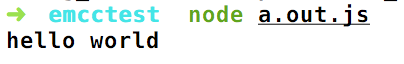
\includegraphics[width=200bp]{figure/pic/hello-world-sample-cli.png}
    \caption{hello world移植程序在cli(node.js)下运行效果}
    \label{hello-world-sample-cli}
\end{figure}

图\ref{hello-world-sample-html}展示了移植程序在浏览器中运行的效果。

\begin{figure}[h!] % [h!] 表示尽量排在当前位置
    \centering
    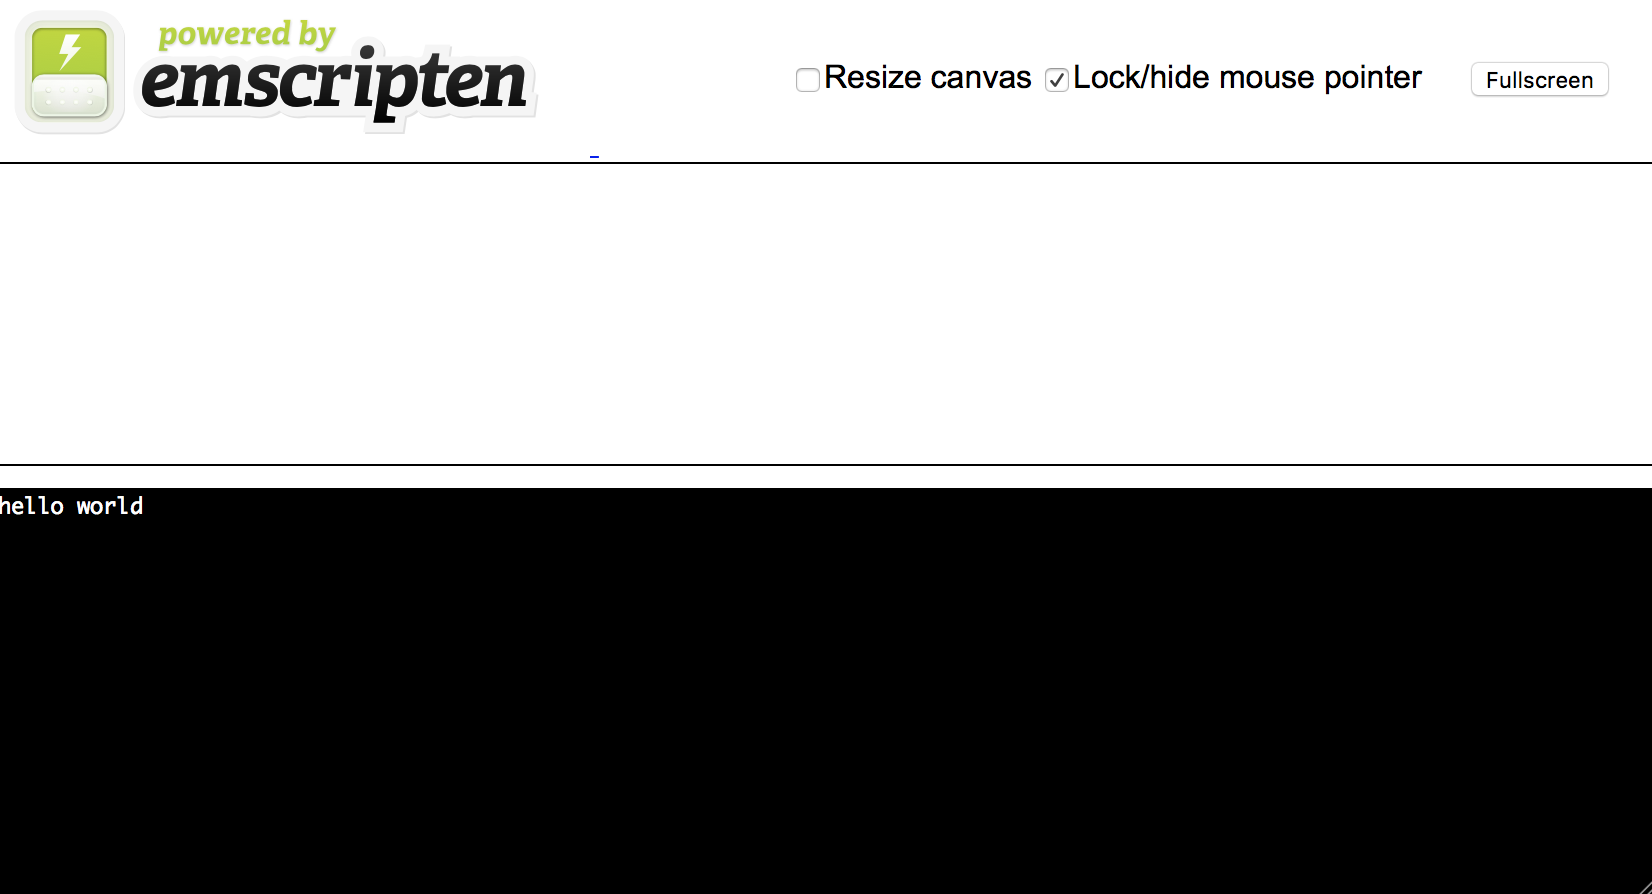
\includegraphics[width=400bp]{figure/pic/hello-world-sample-html.png}
    \caption{hello world移植程序在浏览器中运行效果}
    \label{hello-world-sample-html}
\end{figure}

\section{lua virtual machine 移植过程}

移植lua virtual machine非常简单,顺畅。

\subsection{lua移植过程}

\begin{enumerate}
    \item 下载lua源代码,我使用的是lua 5.2.4版本。
    \item 在lua源代码目录下执行\ref{bash-luavm}命令
        \begin{lstlisting}[
    		language={bash},
    		caption={lua程序的源代码编译命令},
    		label={bash-luavm},
		]

		make emscripten
		\end{lstlisting}
	\item 得到lua.vm.js文件
\end{enumerate}

{\heiti 解释 : } make emscripten是emscripten工具集给的一个简易扩展命令,可以告诉make工具,
使用emcc代替makefile中定义的C/C++编译器

\subsection{lua交互式解释器代码}

下面\ref{html-lua-repl}是lua在线REPL(Read eval print loop)的关键代码

\begin{lstlisting}[
    language={html},
    caption={lua REPL关键代码},
    label={html-lua-repl},
]

<!DOCTYPE html>
<html lang="en">
  <head>
    <meta charset="utf-8">
    <title>lua.vm.js REPL</title>
    <meta name="viewport" content="width=device-width, initial-scale=1.0">
    <meta name="description" content="">
    <meta name="author" content="">

    <!-- Le styles -->
    <link href="css/bootstrap.css" rel="stylesheet">
    <style>
      body {
        padding-top: 60px; /* 60px to make the container go all the way to the bottom of the topbar */
      }
    </style>
    <link href="css/bootstrap-responsive.css" rel="stylesheet">

    <!-- HTML5 shim, for IE6-8 support of HTML5 elements -->
    <!--[if lt IE 9]>
      <script src="js/html5shiv.js"></script>
    <![endif]-->

    <!-- codemirror -->
    <script src="js/codemirror.js"></script>
    <link rel="stylesheet" href="css/codemirror.css">
    <script src="js/lua.js"></script>

  </head>

  <body>

    <div class="navbar navbar-inverse navbar-fixed-top">
      <div class="navbar-inner">
        <div class="container">
          <button type="button" class="btn btn-navbar" data-toggle="collapse" data-target=".nav-collapse">
            <span class="icon-bar"></span>
            <span class="icon-bar"></span>
            <span class="icon-bar"></span>
          </button>
          <a class="brand" href="lua.vm.js.html">lua.vm.js</a>
          <div class="nav-collapse collapse">
            <ul class="nav">
              <li class="active"><a href="repl.html">REPL</a></li>
            </ul>
          </div><!--/.nav-collapse -->
        </div>
      </div>
    </div>

    <div class="container">

      <div class="hero-unit">
        <h2>Lua REPL(交互式解释器)</h2>
        <p>这是一个 Lua 语言的<a href="http://en.wikipedia.org/wiki/Read%E2%80%93eval%E2%80%93print_loop">REPL</a> . 点击按钮执行编辑区域中的代码. 你也可以编写你自己的lua代码并运行.</p>
      </div>

      <div class="row">
        <div class="span7" border=1>
          <textarea id="mytext">
print('hello' .. ' ' .. 'world!') -- This is Lua!

print(js.global:eval('[0,1,2,3,4,5][3]')) -- Run JS from Lua

-- Interact with the page using Lua

local screen = js.global.screen
print("you haz " .. (screen.width*screen.height) .. " pixels")

local window = js.global -- global object in JS is the window
window:alert("hello from lua!")
window:setTimeout(function() print('hello from lua callback') end, 2500)

local document = js.global.document
print("this window has title '" .. document.title .. "'")

-- call constructors (global, or as properties of other objects)
print("i made an ArrayBuffer of size " .. js.new(js.global.ArrayBuffer, 20).byteLength)
-- print("i made an ArrayBuffer of size " .. js.global.ArrayBuffer:new(20).byteLength)

print("time iz " .. js.global.Date.now()) -- call with no arguments

print('done!')
</textarea>
        </div>
        <div class="span5">
          <h4>output</h4>
          <pre id="output"></pre>
        </div>
      </div>

      <p><a href="#" class="btn btn-primary btn-large " onclick="executeLua(myCodeMirror.getValue(), true); return false" id="the_button">Execute &raquo;</a></p>

      <div class="row-fluid">
        <div class="span">
      </div>

    </div> <!-- /container -->

<script>
// CodeMirror
var myCodeMirror = CodeMirror.fromTextArea(document.getElementById('mytext'));
//myCodeMirror.setSize(screen.width*0.6, screen.height*0.2);
// Execution
var outputElement = document.getElementById('output')
var Module = {
  print: function(x) {
    outputElement.textContent = (outputElement.textContent ? outputElement.textContent + '\n' : '') + x;
  }
};
function executeLua(code, clear) {
  if (clear) {
    outputElement.style.color = null;
    outputElement.textContent = '';
  }
  try {
    L.execute(code);
  } catch(e) {
    outputElement.style.color = "red";
    outputElement.textContent = e.toString();
  }
}
</script>

<script src="../dist/lua.vm.js"></script>

  </body>
</html>
\end{lstlisting}

{\heiti 解释 : } CodeMirror的作用是代码高亮。 \href{http://aicdg.com/emscriptenDemos/lua/REPL/repl.html}{这个链接}可以访问的部署到互联网上的lua REPL,可以进行在线测试。

\subsection{lua交互式解释器运行效果}

图\ref{lua-vm-repl}展示了lua REPL在浏览器中运行的效果。

\begin{figure}[h!] % [h!] 表示尽量排在当前位置
    \centering
    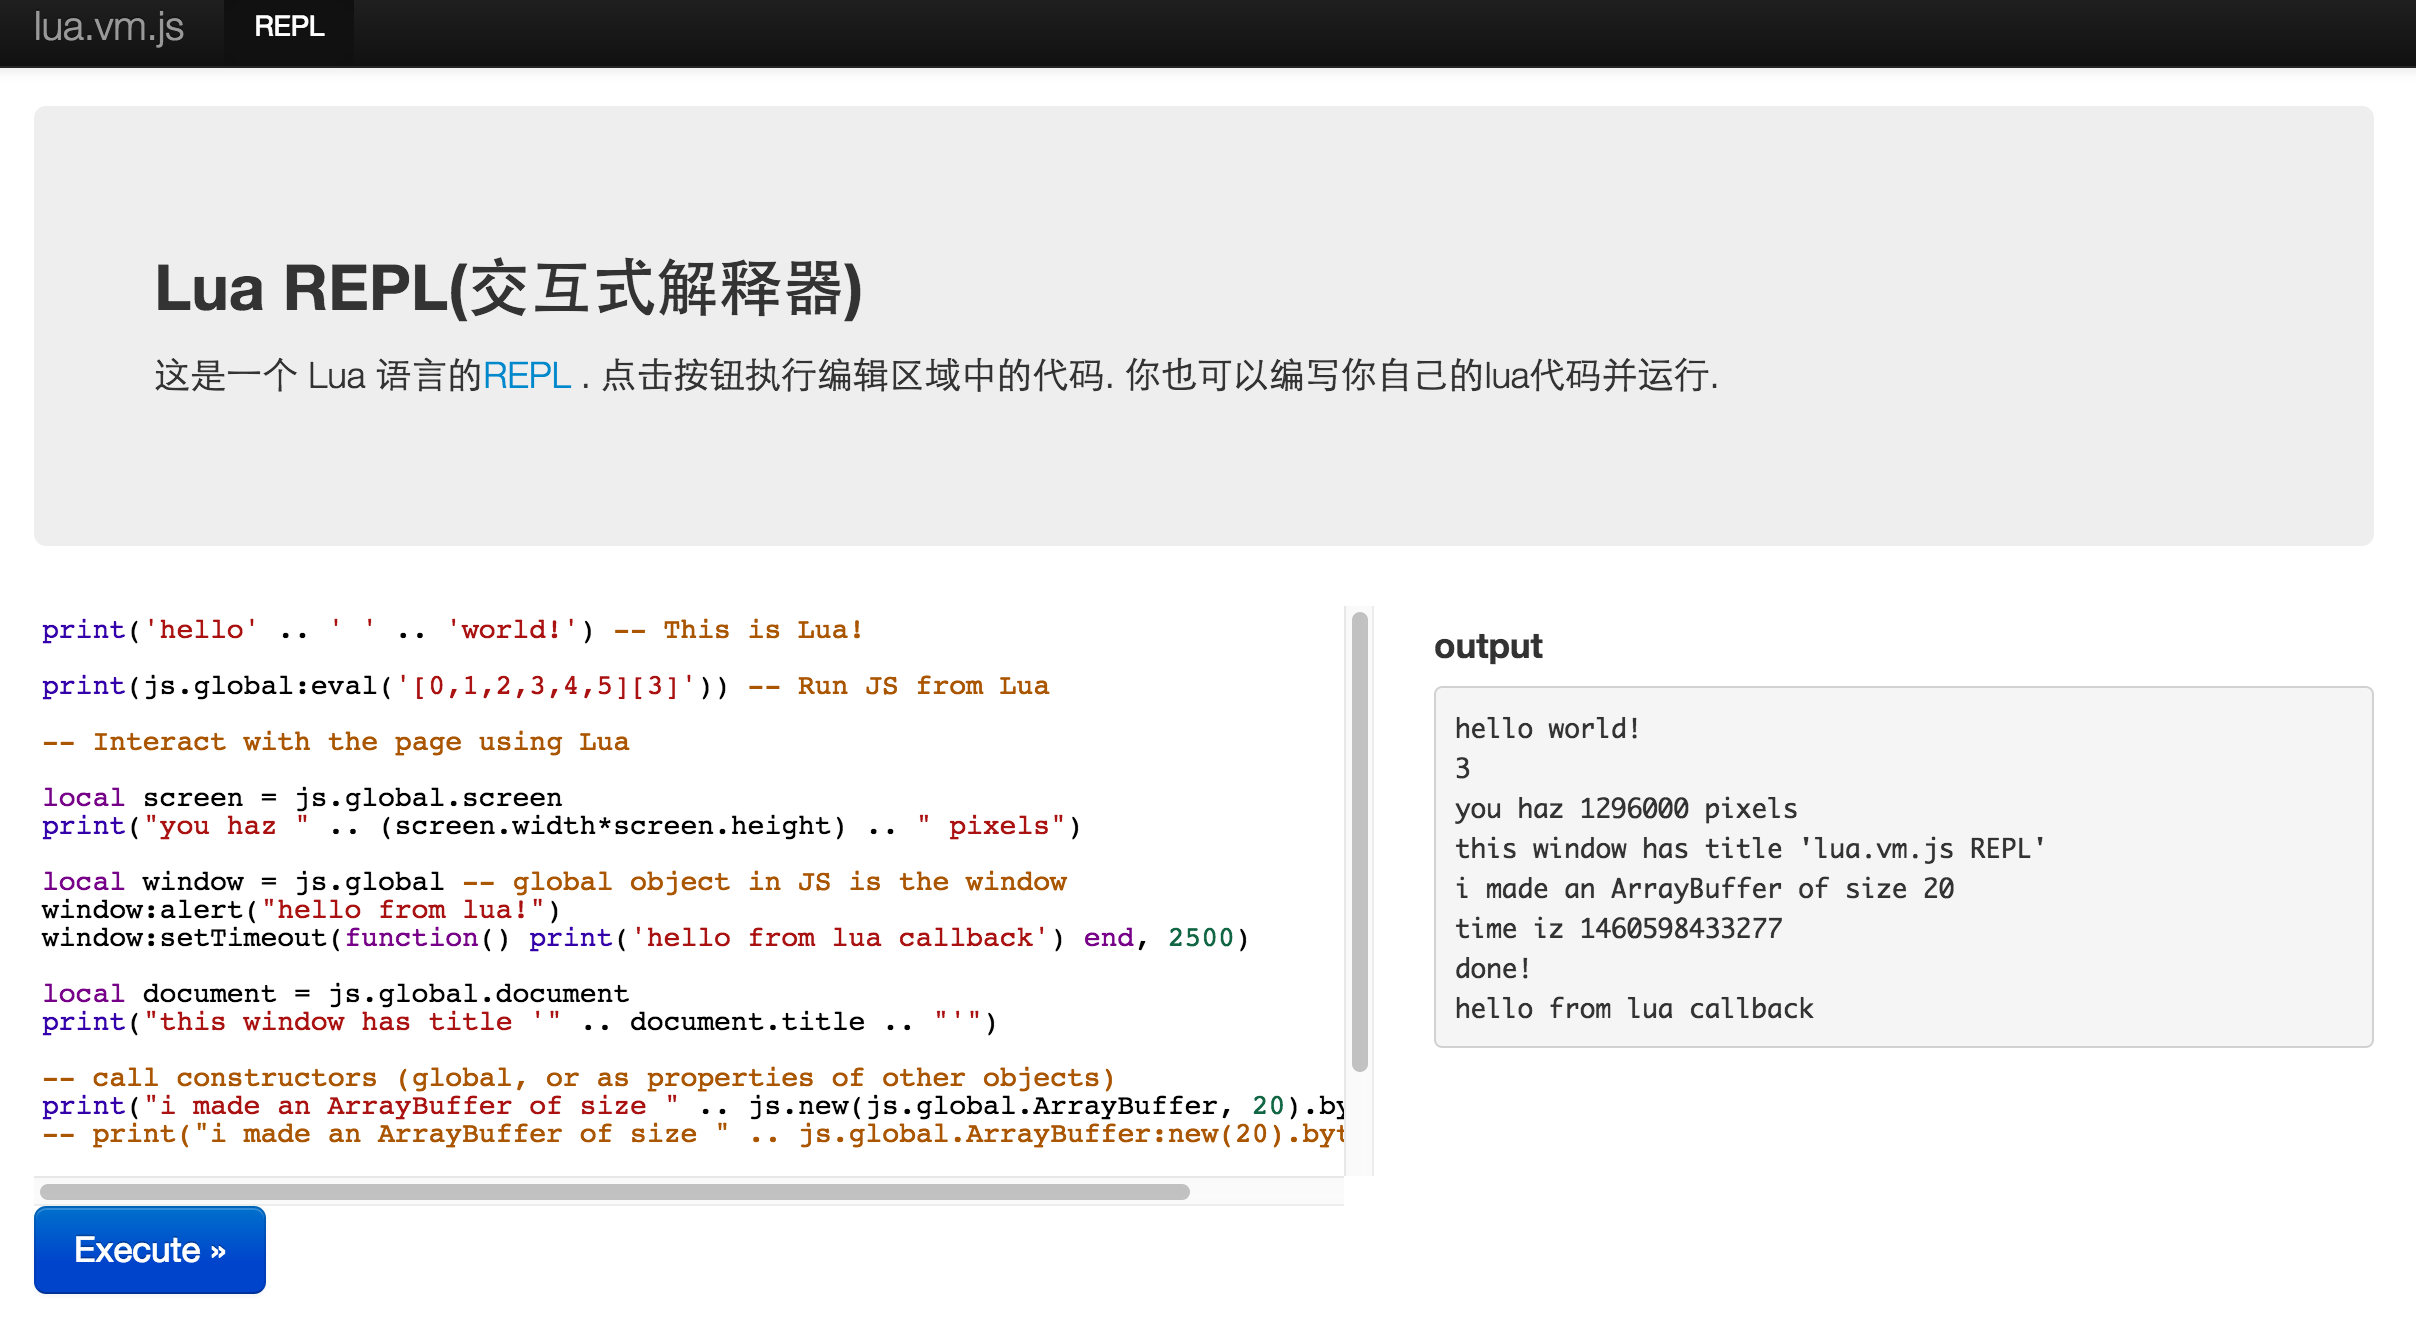
\includegraphics[width=400bp]{figure/pic/lua-vm-repl.png}
    \caption{lua REPL在浏览器中运行效果}
    \label{lua-vm-repl}
\end{figure}